\documentclass[11pt]{article}

\usepackage[margin=1in]{geometry}
\usepackage{amsmath,amssymb}
\usepackage{booktabs}
\usepackage[hidelinks]{hyperref}
\usepackage{tikz}
\usetikzlibrary{arrows.meta,positioning,calc}
\usepackage{graphicx}
\usepackage{float}
\usepackage{booktabs,tabularx,array}

\title{Model Version 1 Outline}
\author{}
\date{}

\begin{document}
\maketitle


\section{Objective}
    The primary object is to use the pre-training plus fine-tuning paradigm, ontop of some kind of transformer 
    architecture. The most obvious choice was to do win-prediction, hence the goal is win prediction. 

    Ultimately, this sub-project is about selecting and justifying an architecture (for the given task, which may 
    not be well posed), and empirically learning about the effects of choices like optimizers, loss functions, 
    regularization techniques, and subtle architecture adjustments. All is in the service of spurring on my own 
    interest in the field.



\section{Data}
    The data for this project comes from a public Deadlock data API. It comes in two forms:
    \begin{enumerate}
        \item End-of-Match - This is essentially a screenshot of the final scoreboard. This will include variables determined by the outcome of the game, like kills, death, items, and souls, but will also have element invariant of outcome, like character selection, lane assignment, and rank (elo).
        \item Event Stream - This is literally the entire game. Every entities position at every tick of the game, every characters soul count, kills, deaths, assists, spatial position, ability cooldowns, etc. This is the ultra-high resolution spatial-temporal data that initial inspired me to consider this dataset.
    \end{enumerate}
    These two datasets provide a nice form factor for the pre-training/fine-tuning paradigm. The first, End-of-Match data, is extremely small, and easy to get, providing the usual medium for pre-training. The second, Event Stream data, provide, again, an excellent structure for this paradigm; Extremely high resolution, expensive, well labeled data. However, the event stream data also has the bonus feature that the ultra-high detail of it allows for multimodal use of the data.



\newpage 
\section{Architecture}
    The architecture I came up with is as follows:
% Final Architecture Layout
    \begin{figure}[H]
    \centering
    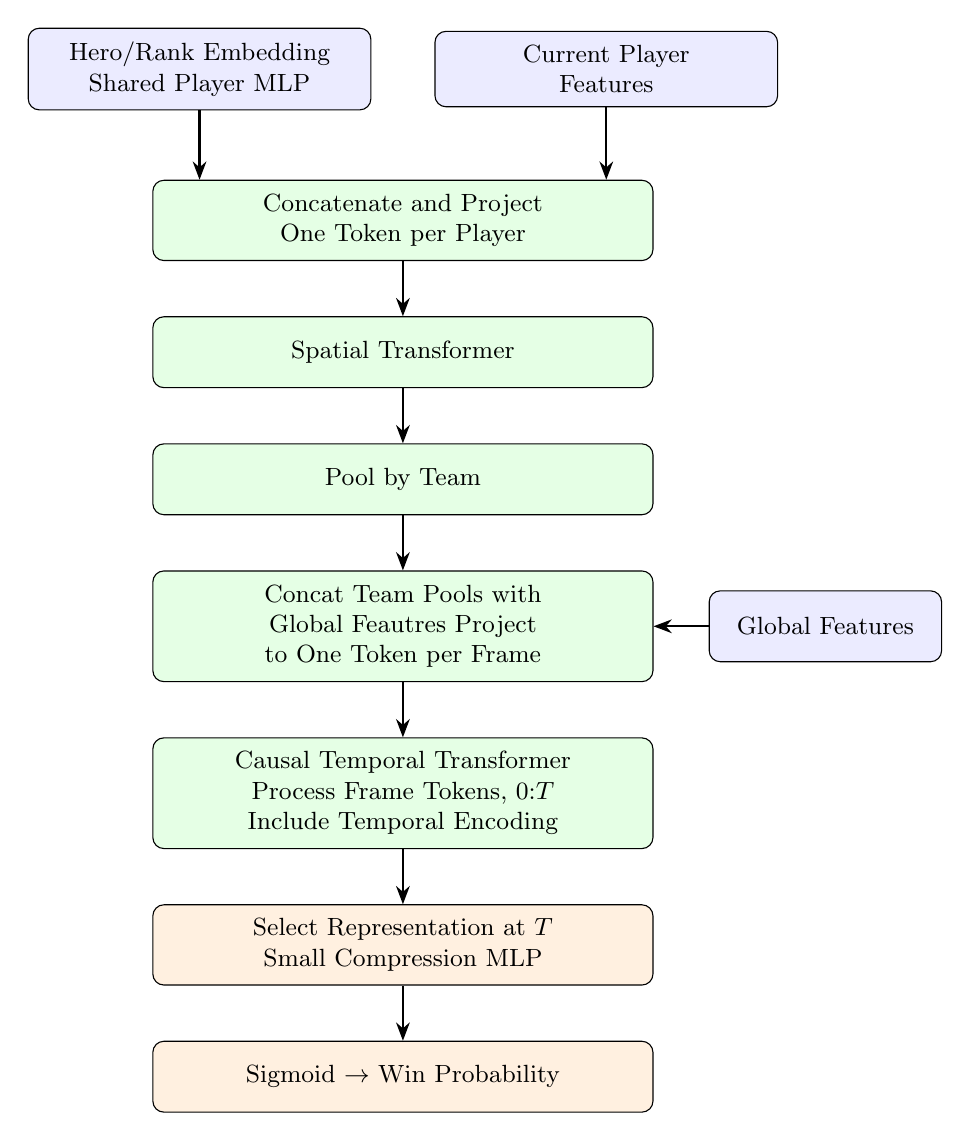
\begin{tikzpicture}[
        font=\small,
        node distance=7mm,
        box/.style={
            draw,
            rounded corners,
            align=center,
            text width=6cm,
            minimum height=9mm,
            inner sep=5pt
        },
        input/.style={box, text width=4cm, fill=blue!8},
        process/.style={box, fill=green!10},
        output/.style={box, fill=orange!12},
        arrow/.style={-{Stealth}, thick}
    ]

    \node[input] (hero) {
        Hero/Rank Embedding\\
        Shared Player MLP
    };

    \node[input, right=8mm of hero] (state) {
        Current Player\\
        Features
    };

    \coordinate (middle) at
        ($(hero.south)!0.5!(state.south)$);

    \node[process, below=9mm of middle] (concat) {
        Concatenate and Project\\
        One Token per Player
    };

    \node[process, below=of concat] (spatial) {
        Spatial Transformer
    };

    \node[process, below=of spatial] (pool) {
        Pool by Team
    };

    \node[process, below=of pool] (frame) {
        Concat Team Pools with\\
        Global Feautres
        Project to One Token per Frame
    };

    \node[input, right=7mm of frame, text width=2.6cm] (global) {
        Global Features
    };

    \node[process, below=of frame] (temporal) {
        Causal Temporal Transformer\\
        Process Frame Tokens, $0{:}T$\\
        Include Temporal Encoding
    };

    \node[output, below=of temporal] (head) {
        Select Representation at $T$\\
        Small Compression MLP
    };

    \node[output, below=of head] (win) {
        Sigmoid $\rightarrow$ Win Probability
    };

    \draw[arrow] (hero.south) --
        (concat.north -| hero.south);
    \draw[arrow] (state.south) --
        (concat.north -| state.south);
    \draw[arrow] (concat) -- (spatial);
    \draw[arrow] (spatial) -- (pool);
    \draw[arrow] (pool) -- (frame);
    \draw[arrow] (global.west) -- (frame.east);
    \draw[arrow] (frame) -- (temporal);
    \draw[arrow] (temporal) -- (head);
    \draw[arrow] (head) -- (win);

    \end{tikzpicture}
    \caption{
        Win-prediction architecture.
        Shared player encoding and spatial attention are applied
        to each frame; temporal attention combines the observed
        history to predict the final match outcome.
    }
    \label{fig:final-architecture}
    \end{figure}
\newpage
% Symbolic descriptions
    Let $\mathcal{I}$ denote the set of heroes, e.g., $\mathcal{I}=\{\text{Abrams},\text{Apollo},\text{Warden},\ldots\}$. For a given match, let $p\in\{1,\ldots,12\}$ index players and $t\in\{0,\ldots,T\}$ index observed frames. Player $p$ selects hero $i_p\in\mathcal{I}$ and has scaled pre-match rank $r_p\in\mathbb{R}_+$. Let $\mathbf{x}_{p,t}\in\mathbb{R}^{F}$ contain current player features, including team identity, position, kills and death, and let $\mathbf{g}_t\in\mathbb{R}^{G}$ contain global features like tower damage, urn count, elasped time. Let $[\mathbf{a};\mathbf{b}]$ denote vector concatenation.
% Architectural description
    \begin{table}[H]
    \centering
    \small
    \renewcommand{\arraystretch}{1.3}
    \setlength{\tabcolsep}{5pt}

    \begin{tabularx}{\textwidth}{
        >{\raggedright\arraybackslash}p{0.20\textwidth}
        >{\raggedright\arraybackslash}X
        >{\raggedright\arraybackslash}p{0.44\textwidth}
    }
    \toprule
    \textbf{Component} &
    \textbf{Purpose} &
    \textbf{Symbol \& Structure} \\
    \midrule

    Hero embedding &
    Learned hero lookup vector. &
    $e_i \in \mathbb{R}^{16}$ for each $i \in \mathcal{I}$\\

    Static player MLP &
    Condition hero representation on rank. &
    $\mathbf{s}_p=f_{\mathrm{static}}([\mathbf{e}_{i_p};r_p]) \in\mathbb{R}^{32}$ where $f_{\mathrm{static}}$ is an MLP with ReLU layers
    MLP: $17\rightarrow32\rightarrow32$\\

    Player projection &
    Combine static and current features. &
    $\mathbf{z}_{p,t} =\mathbf{W}_{\mathrm{player}} [\mathbf{s}_p;\mathbf{x}_{p,t}] +\mathbf{b}_{\mathrm{player}} \in\mathbb{R}^{64}$\\

    Spatial transformer &
    Contextualize players within a frame. &
    $\mathbf{U}_t =\operatorname{Spatial}(\mathbf{Z}_t) \in\mathbb{R}^{12\times64}$; 1 block, 4 heads, feed-forward with width 128. \\

    Team pooling &
    Summarize each team's players. &
    $\displaystyle\mathbf{a}_{k,t}=\frac{1}{6}\sum_{p\in\mathcal{P}_k}\mathbf{u}_{p,t}\in\mathbb{R}^{64}$, where $\mathcal{P}_k$ is team $k$'s player set. \\

    Frame projection &
    Combine team summaries and global state. &
    $\mathbf{v}_t=\mathbf{W}_{\mathrm{frame}}[\mathbf{a}_{1,t};\mathbf{a}_{2,t};\mathbf{g}_t]+\mathbf{b}_{\mathrm{frame}}\in\mathbb{R}^{64}$. \\

    Temporal encoding &
    Represent frame order. &
    $\tilde{\mathbf{v}}_t=\mathbf{v}_t+\mathbf{q}_t$, where $\mathbf{q}_t\in\mathbb{R}^{64}$ is a positional encoding. \\

    Temporal transformer &
    Represent observed match history. &
    $\mathbf{h}_T=\operatorname{Temporal}(\tilde{\mathbf{v}}_0,\ldots,\tilde{\mathbf{v}}_T)_T\in\mathbb{R}^{64}$; 2 blocks, 4 heads, feed-forward with width 128. \\

    Win head &
    Predict team 1's win probability. &
    $\hat{p}_T=\sigma(f_{\mathrm{win}}(\mathbf{h}_T))$; where $f_{\mathrm{win}}$ is an MLP with ReLU layers $64\rightarrow32\rightarrow1$\\

    \bottomrule
    \end{tabularx}

    \caption{
        Proposed architecture.
        $\mathbf{Z}_t$ stacks player tokens as rows;
        $\mathbf{u}_{p,t}$ is player $p$'s spatial output.
    }
    \label{tab:model-components}
    \end{table}
    Now with the architecture figured out, how to train it becomes the next major question.


\newpage
\section{Training}
    In order to meet the goals of this sub-project, and take advantage of all the available data, this is the following training procedure I have come up with for this model. Note that numerical values for parameters are intial quantities and will likely be adjusted during training.
% Graph of training order
    \begin{figure}[H]
    \centering
    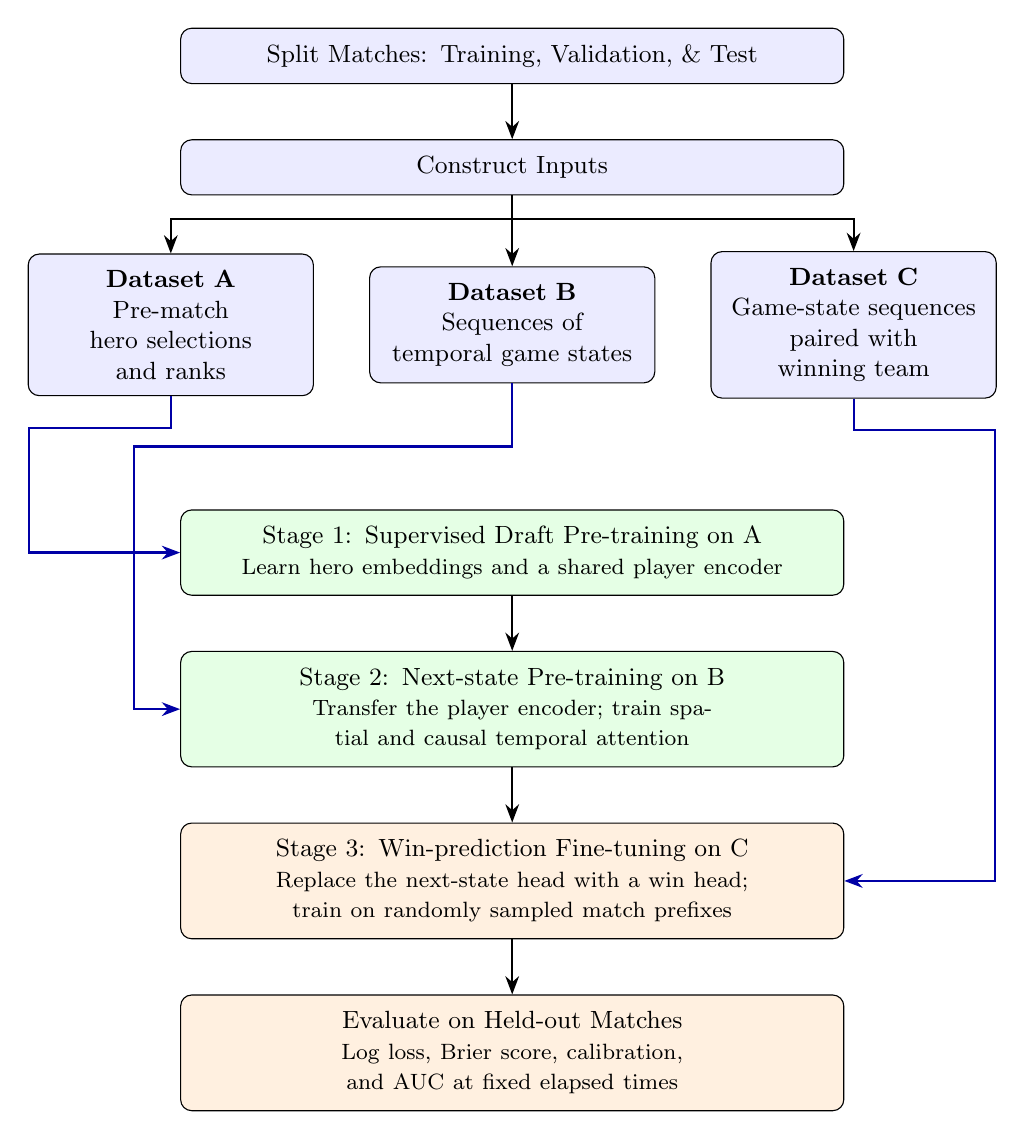
\begin{tikzpicture}[
        font=\small,
        node distance=7mm,
        box/.style={
            draw,
            rounded corners,
            align=center,
            text width=8cm,
            inner sep=6pt
        },
        data/.style={box, fill=blue!8},
        dataset/.style={data, text width=3.2cm, minimum height=1.2cm},
        train/.style={box, fill=green!10},
        final/.style={box, fill=orange!12},
        arrow/.style={-{Stealth}, thick},
        feed/.style={arrow, blue!65!black}
    ]

    \node[data] (split) {
        Split Matches: Training, Validation, \& Test
    };

    \node[data, below=of split] (inputs) {
        Construct Inputs
    };

    % Three dataset branches.
    \node[dataset, below=9mm of inputs] (B) {
        \textbf{Dataset B}\\
        Sequences of \\temporal game states
    };

    \node[dataset, left=7mm of B] (A) {
        \textbf{Dataset A}\\
        Pre-match hero selections\\
        and ranks
    };

    \node[dataset, right=7mm of B] (C) {
        \textbf{Dataset C}\\
        Game-state sequences\\
        paired with winning team
    };

    % Training stages.
    \node[train, below=16mm of B] (stage1) {
        Stage 1: Supervised Draft Pre-training on A\\
        \footnotesize
        Learn hero embeddings and a shared player encoder
    };

    \node[train, below=of stage1] (stage2) {
        Stage 2: Next-state Pre-training on B\\
        \footnotesize
        Transfer the player encoder;
        train spatial and causal temporal attention
    };

    \node[final, below=of stage2] (stage3) {
        Stage 3: Win-prediction Fine-tuning on C\\
        \footnotesize
        Replace the next-state head with a win head;
        train on randomly sampled match prefixes
    };

    \node[final, below=of stage3] (evaluate) {
        Evaluate on Held-out Matches\\
        \footnotesize
        Log loss, Brier score, calibration, and AUC
        at fixed elapsed times
    };

    % Input construction branches.
    \draw[arrow] (split) -- (inputs);
    \draw[arrow] (inputs.south) -- (B.north);
    \draw[arrow] (inputs.south) -- ++(0,-3mm) -| (A.north);
    \draw[arrow] (inputs.south) -- ++(0,-3mm) -| (C.north);

    % Dataset A enters Stage 1 from the left.
    \draw[feed] (A.south)
        -- ++(0,-4mm)
        -- ++(-1.8cm,0)
        |- (stage1.west);

    % Dataset B enters Stage 2 via a separate left-hand route.
    \draw[feed] (B.south)
        -- ++(0,-8mm)
        -- ++(-4.8cm,0)
        |- (stage2.west);

    % Dataset C enters Stage 3 from the right.
    \draw[feed] (C.south)
        -- ++(0,-4mm)
        -- ++(1.8cm,0)
        |- (stage3.east);

    % Sequential parameter transfer and evaluation.
    \draw[arrow] (stage1) -- (stage2);
    \draw[arrow] (stage2) -- (stage3);
    \draw[arrow] (stage3) -- (evaluate);

    \end{tikzpicture}
    \caption{
        Proposed training procedure.
        Blue arrows supply each stage with its corresponding dataset;
        black arrows between training stages indicate parameter and data transfer.
        Datasets B and C may use the same trajectories,
        with different training targets.
    }
    \label{fig:training-procedure}
    \end{figure}
    using this high-level overview, I now consider each step in more detail.

    \subsection{Pre-Train 1 - Static Embeddings}
        The goal of this pre-training stage is to learn hero embeddings and a shared MLP that combines hero identity with pre-match rank. These components produce static player representations that are transferred to the subsequent training stages.
    \subsubsection{Architecture}
% Detailed graph of training architecture for embedding pre-train
        \begin{figure}[H]
        \centering
        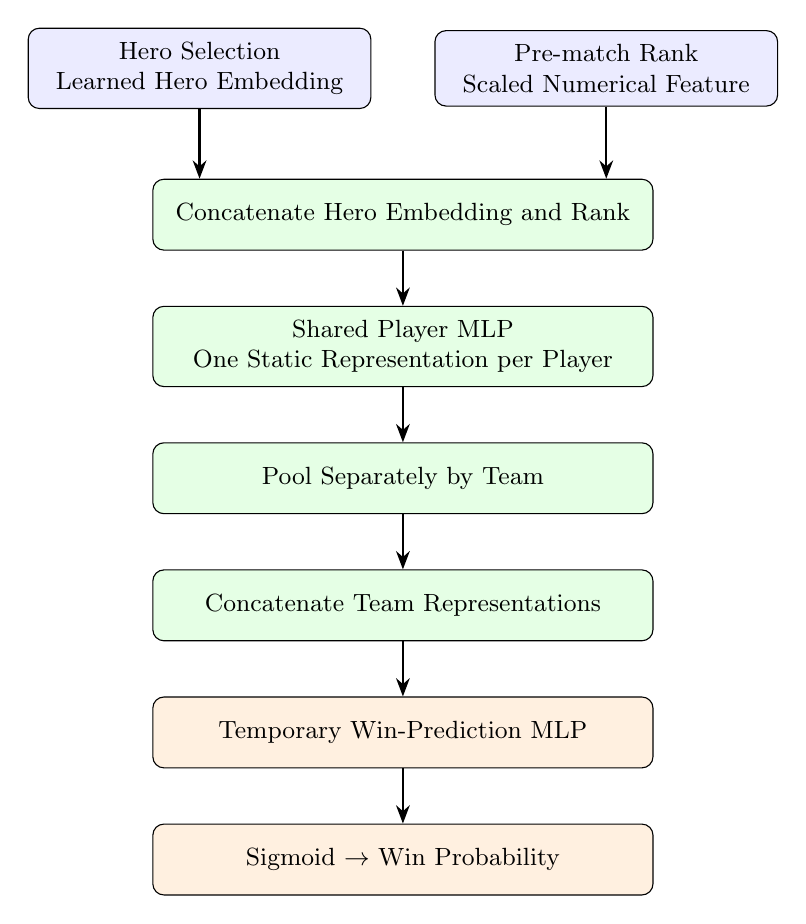
\begin{tikzpicture}[
            font=\small,
            node distance=7mm,
            box/.style={
                draw,
                rounded corners,
                align=center,
                text width=6cm,
                minimum height=9mm,
                inner sep=5pt
            },
            input/.style={box, text width=4cm, fill=blue!8},
            process/.style={box, fill=green!10},
            output/.style={box, fill=orange!12},
            arrow/.style={-{Stealth}, thick}
        ]

        \node[input] (hero) {
            Hero Selection\\
            Learned Hero Embedding
        };

        \node[input, right=8mm of hero] (rank) {
            Pre-match Rank\\
            Scaled Numerical Feature
        };

        \coordinate (middle) at
            ($(hero.south)!0.5!(rank.south)$);

        \node[process, below=9mm of middle] (concat) {
            Concatenate Hero Embedding and Rank
        };

        \node[process, below=of concat] (static) {
            Shared Player MLP\\
            One Static Representation per Player
        };

        \node[process, below=of static] (pool) {
            Pool Separately by Team
        };

        \node[process, below=of pool] (teams) {
            Concatenate Team Representations
        };

        \node[output, below=of teams] (head) {
            Temporary Win-Prediction MLP
        };

        \node[output, below=of head] (win) {
            Sigmoid $\rightarrow$ Win Probability
        };

        \draw[arrow] (hero.south) --
            (concat.north -| hero.south);
        \draw[arrow] (rank.south) --
            (concat.north -| rank.south);
        \draw[arrow] (concat) -- (static);
        \draw[arrow] (static) -- (pool);
        \draw[arrow] (pool) -- (teams);
        \draw[arrow] (teams) -- (head);
        \draw[arrow] (head) -- (win);

        \end{tikzpicture}
        \caption{
            Draft-based pre-training architecture.
            Hero embeddings and the shared player MLP are trained
            using match outcomes and transferred to Stage 2.
            Everything after the pooling is discarded.
        }
        \label{fig:pretrain1-architecture}
        \end{figure}

    \subsubsection{Loss function}
        Since this is a win-prediction task, I use binary cross-entropy between prediect probability that team 1 wins and the observed outcome. For the same of numerical stability, loss is computed directly from the output logit using \texttt{BCEWithLogitsLoss}.
    \subsubsection{Optimizer and learning rate}
        I use AdamW with an initial learning rate of $10^{-3}$ and weight decay of $10^{-4}$. These are starting values, an may be adjusted later based on validation loss.

    \subsubsection{Batch size and training duration}
        I use mini-batches of 64 matches and will train for at most 100 epochs, shuffling the training matches at each epoch. I retain the checkpoint with the lowest validation binary cross-entropy.

    \subsubsection{Regularization and stopping criteria}
        I halt if the validation loss does not improve for 10 consecutive epochs. Initially, I do not use dropouts but this may change if training loss continues to decrease while validation loss worsens. Similarly, I initially do not use weight decay, but in the event of overfitting, I will.

\subsection{Pre-Train 2 - Temporal Dyanmics}

\subsection{Fine-Tune - Win Prediction}







\section{Evaluation}

\section{Open Questions}
This architecture incorporates all the targeted, non-mutually exclusive, methods I wanted to exercise:
\begin{itemize}
    \item \textbf{Embeddings} - Learned one-hot hero embeddings (like text) with numeric information, rank, to compose a composit embedding.
    \item \textbf{Transformers} - Using both spatial and temporal attention with different structures.
    \item \textbf{Parameter sharing} - Using the parameters from one model, or training, inside of another.
    \item \textbf{Residuals \& Layer Normalizing} - Considerations for regularizing magnitudes, normalizing values between layers for training stability.
    \item \textbf{Causal Masking \& Temporal Encoding} - Temporal encoding for game state flow, and causul masking to preserve temporal information flow.
    \item \textbf{Supervised Pre-Training} - Using high-quantity labeled data to learn embeddings.
    \item \textbf{Self-Supervised Pre-Training} - Using temporal game-state data to learn game dynamics.
    \item \textbf{Transfer Learning \& Fine-Tuning} - Pre-trained components are reused as trained representation generation for win prediction.
    \item \textbf{Random-Prefix Training} - Randomly cut temporal observations to train model prediction outs over variable time horizons.
\end{itemize}


\end{document}
